\chapter{Trajectory patterns}\label{trajectories}
\section{Introduction}
This GSP attempts to identify people's movement patterns from anonymized Wi-Fi logs. \Cref{movements} described movement patterns including spatial and temporal aspects of single movements of a crowd of people. Another way of looking at movements, is by tracking individual movement for a longer time interval. A large set of individual trajectories can be used for the identification of typical movements among users of the campus. The method uses concepts from sequential pattern mining. \\\\
This chapter presents a method for identifying movement patterns using individual trajectories. As described in \autoref{movementpatterns}, if moving individuals share some locations in their trajectory, you can speak of co-location in space. When the order of the shared locations are similar for multiple trajectories, you can speak of typical movement. This concept is explored for the identification of movement patterns, and thus the usage of the campus. This approach can answer different questions than looking at single movements, as is done in \autoref{movements}. For example, ‘how many places the user frequently visits’, ‘at what order the user visits places’, ‘how often a trajectory happens’, ‘how many places contained in a frequent trajectory’.\\\\
First, this chapter will describe the problem description, including the extraction of locations of a user, the mining of individual trajectories from an anonymized Wi-Fi scan list, and finally the mining of movement patterns from a set of trajectories using the PrefixSpan algorithm.
\section{Problem description}
The data provided by the eduroam network enables a detailed view of people's movement on campus. The large coverage of the eduroam network allows to track users for a large part of the day when they enter the campus. However, the observation space is limited to the extent of the size of the campus, making it not possible to track people outside the eduroam network. A second disadvantage is the spatial resolution of the positioning method. The range a mobile device can be connected to an AP,  influences the accuracy of the estimated location of a mobile device. For indoor environments of the TU Delft campus, this is just a few tens of meters wide. This resolution allows tracking movement at a building level by re-locating mobile devices to the closest AP. Data between two re-locations is not available. Therefore, an individual's trajectory is depicted by connecting the re-locations as a sequence of APs. These individual trajectories are used to identify patterns. \\\\
A location represents a geographic position where a user stays, i.e. a user is in state. For identifying movement patterns from Wi-Fi monitoring, we are interested in movement between two locations where an individual stays for a longer time period. Such a location, or stay place, can be detected when a user is connected to the same AP for a longer time. To detect  buildings as a location (i.e. contains multiple APs), two consecutive Wi-Fi scans must contain  APs of the same building. With a data collecting interval of 5 minutes, it means that people will be filtered out if their stay duration is less than 10 minutes. Based on this assumption, people with a shorter stay duration are considered passing by, as explained in \autoref{preprocessing}.

\subsection{Trajectory Pattern}
An individual's trajectory is constructed as a sequence of locations in order of the scan time. 
$$p_{1} \rightarrow p_{2} \rightarrow p_{3} \rightarrow …\rightarrow p_{n}$$
From a set \textit{S} of trajectories, different patterns can be identified using sequential pattern mining algorithms. Frequency of a trajectory by all users of the campus can be detected. This can be represented as a trajectory \textit{T} with a support \textit{s}. Support means how many times the same sequence, or sub-sequence, is shared in the set of trajectories. This gives valuable information on the order common buildings are used and what order of buildings occurs the most. Using a minimum support threshold, sequential mining returns all movement patterns that satisfy \textit{n} \textgreater 2 and support \textit{T} \textgreater \textit{$S_{min}$}   Furthermore, the length of common trajectories can be discovered. This allows for identification of movement patterns of a specific length \textit{n}. Also, when location is not considered, but only the length of a trajectory, the mobility pattern of an individual can be described in terms of how many times he/she re-locates. \autoref{figure:figseqpattern} illustrates a trajectory pattern of length 3, and has a support of 3.

\begin{figure}[H]
\centering
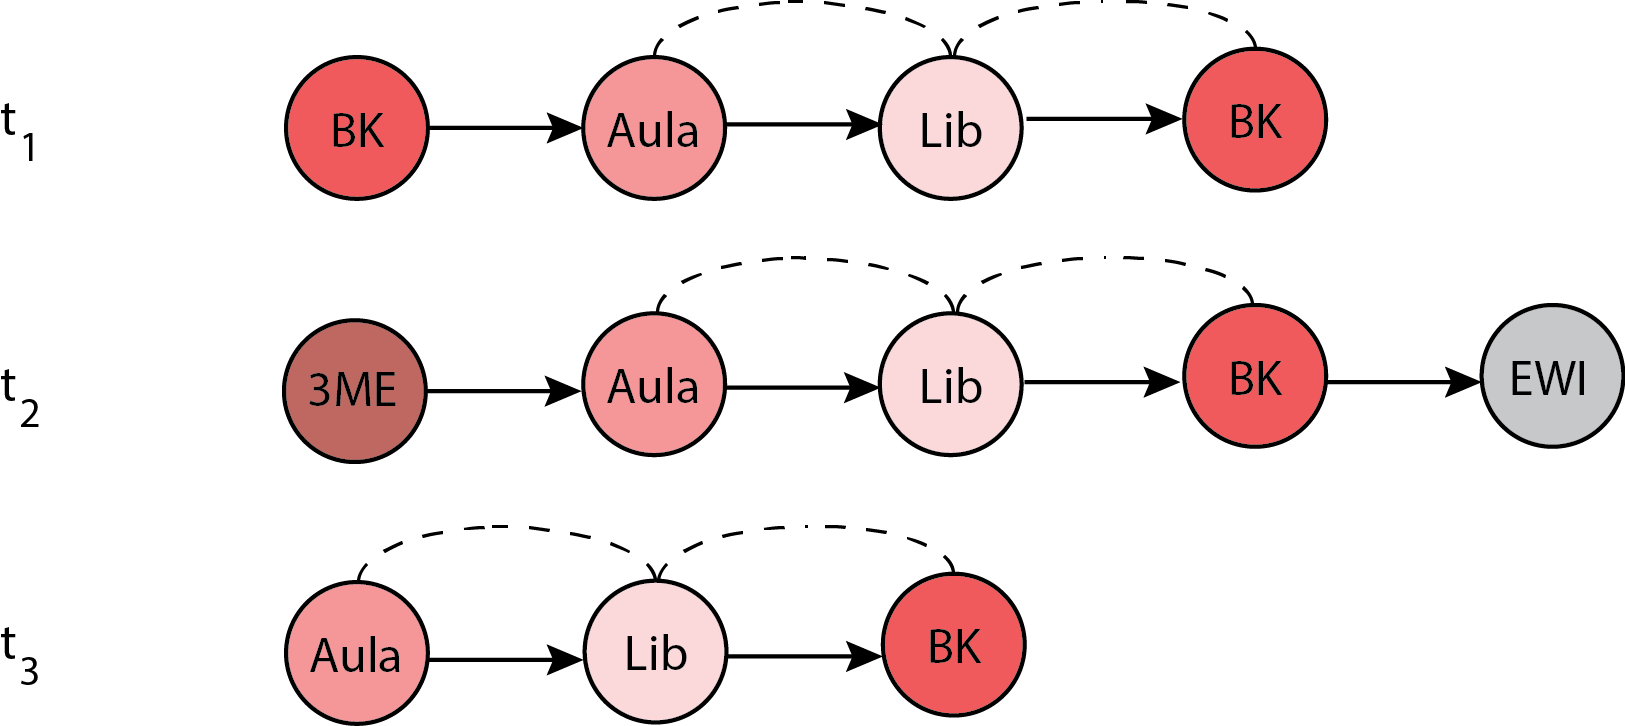
\includegraphics[scale=0.6]{sub-sequence-pattern.png}
\captionsetup{justification=centering}
\caption{trajectories of three days, and the trajectory pattern}
\label{figure:figseqpattern}
\end{figure}
For this study, a trajectory pattern is a sequence of states with \textit{n} \textgreater 2 and support \textgreater \textit{$S_{min}$}. We are only considering trajectory patterns with \textit{n} \textgreater 2, because \autoref{movements} already looked at two consecutive states.\\\\
There exists many developed sequential pattern mining algorithms. For this study PrefixSpan \cite{pei2004mining} is used to identify common shared trajectories or sub-trajectories. This sequential pattern mining algorithm can find re-occurring sequences or sub-sequences from a set of trajectories. For every common sequence, a support value is computed. 
\section{Implementation}
For this analyses the same data is used as for the single movement analysis. As described in \autoref{preprocessing}, from the raw Wi-Fi log states are extracted. More than 2.8 million states are identified from the dataset. This information is stored including a unique mac address, a number representing a building, the start time of the state and the end time of the state. The states are used to construct individual sequences ordered by date and time. The \textit{$T_{split}$} is used to create separate trajectories for different days, for each individual. For this study, a new trajectory is created when there has not been a connection for 5.5 hours, i.e. a state of outside campus ('world') > 5.5 hours. This threshold is suitable for identifying people moving home at the end of the day and coming back the next morning. After splitting the sequences, over 950.000 trajectories are created, with temporal granularity of one day. Every trajectory starts and ends with 'world', i.e. people start and end there trajectory outside the campus. A sample of a constructed trajectory can be seen in \autoref{figure:figtrajectory}

\begin{figure}[H]
\centering
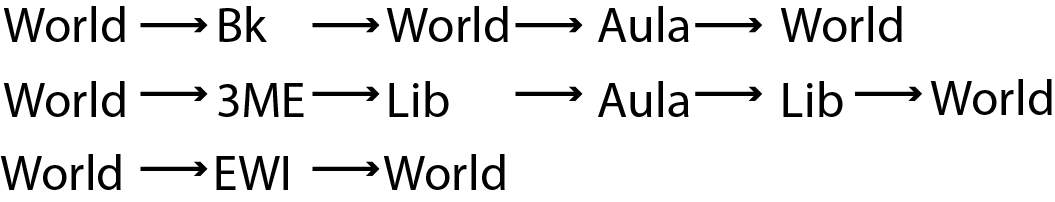
\includegraphics[scale=0.7]{sampleTraject.png}
\captionsetup{justification=centering}
\caption{sample of individual trajectories}
\label{figure:figtrajectory}
\end{figure}
Based on the created trajectories, trajectory patterns with a support value are detected by applying the PrefixSpan algorithm. \autoref{figure:prefixspan} shows an example of the detection of patterns with a support value given by the sequential pattern algorithm. Logically, the pattern with the highest support is a length-1 sequence. The longer patterns get, the lower the support will be.  

\begin{figure}[H]
\centering
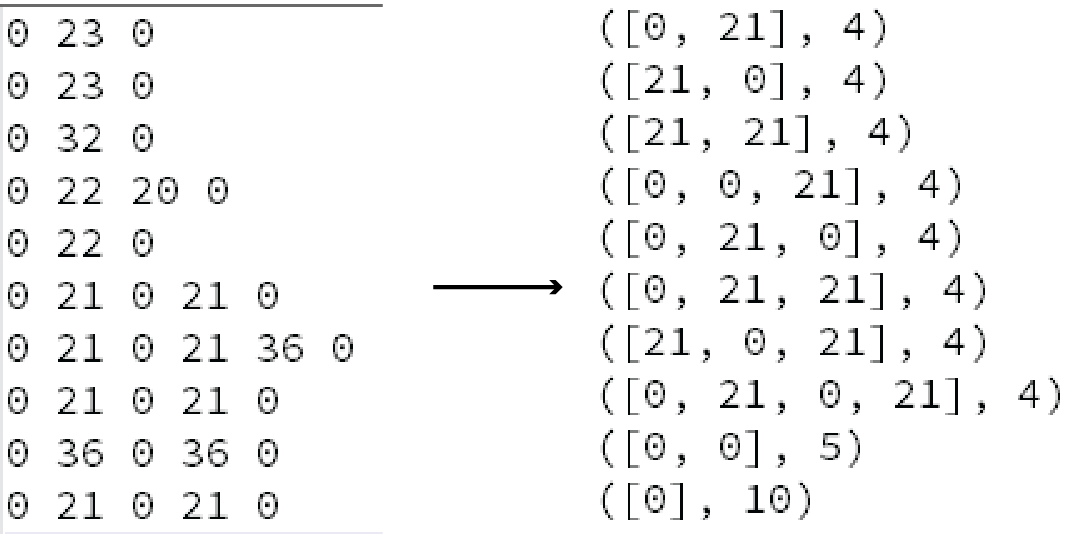
\includegraphics[scale=0.7]{prefixspan.png}
\captionsetup{justification=centering}
\caption{sequential pattern mining sample}
\label{figure:prefixspan}
\end{figure}


\section{Results of trajectory pattern identification}
This section describes the result of the trajectory pattern mining. We used trajectories of mobile devices only, see \autoref{mobility}. 
\subsection{Length of pattern}
From the individual trajectories, the length can be retrieved. This trajectory length is plotted in a histogram, showing how many different places users visit during a day. \autoref{figure:lenhisto} shows that most trajectories consist of three states, i.e. entering the campus, visit one building and leave the campus. The average number of states in a single trajectory is 3.95, this provides information about movement behaviour of users on the campus. 

\begin{figure}[H]
\centering
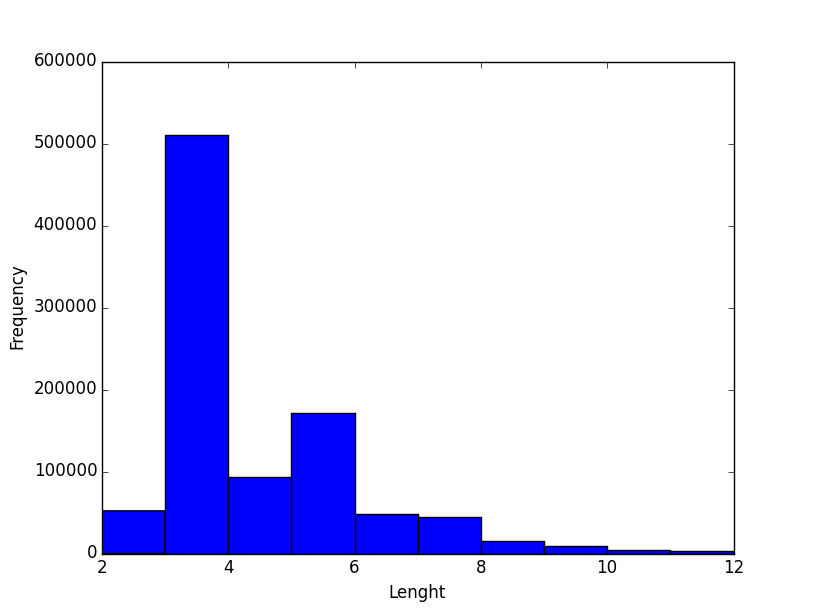
\includegraphics[scale=0.4]{length_histogram.png}
\captionsetup{justification=centering}
\caption{length of individual trajectories as a sequence of states at buildings}
\label{figure:lenhisto}
\end{figure}
In the same way, trajectories at the spatial level of inside a building can be analysed. In \autoref{indoormovement} more on indoor movement is discussed. We analysed the trajectories of individual users inside the Faculty of Architecture and the built environment. The length of more than 150.000 trajectories is plotted in \autoref{figure:lenhistoindoor}. This figure shows, compared to \autoref{figure:lenhisto}, that people visit more different places indoor, than the number of different buildings, i.e. people are more mobile inside the Faculty of Architecture compared to movement between buildings. The average number of states in a single trajectory inside the Faculty of Architecture is 4.66

\begin{figure}[H]
\centering
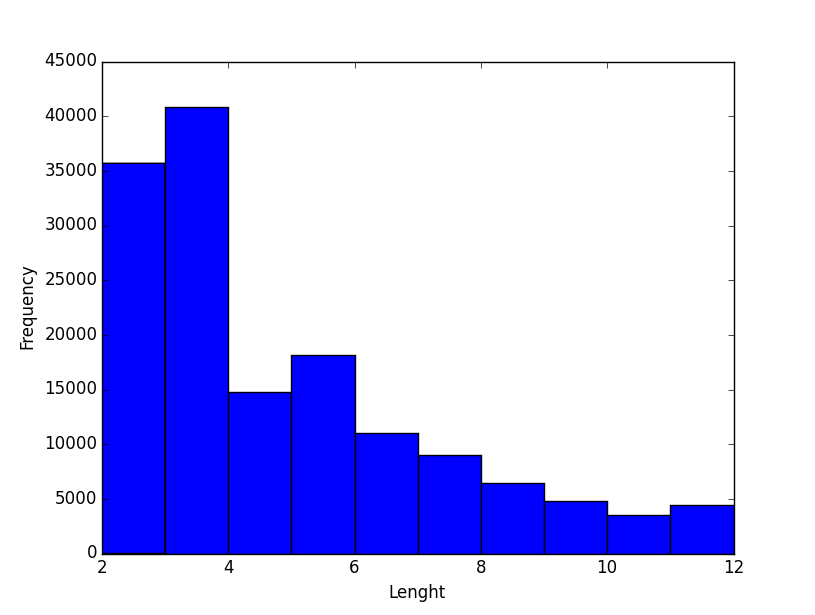
\includegraphics[scale=0.4]{length_histogram_indoor.png}
\captionsetup{justification=centering}
\caption{length of individual trajectories as a sequence of states at indoor building-parts}
\label{figure:lenhistoindoor}
\end{figure}

\subsection{trajectory length-4 pattern}
For the identification of trajectory patterns, we used the trajectories from the building spatial level. To retrieve information about the most common order of at least four distinct locations, we only considered trajectory patterns with a length of four and longer, including 'world'. The three most frequent used order of four distinct locations with support > 1000 is shown in \autoref{figure:len4pattern}.

\begin{figure}[H]
\centering
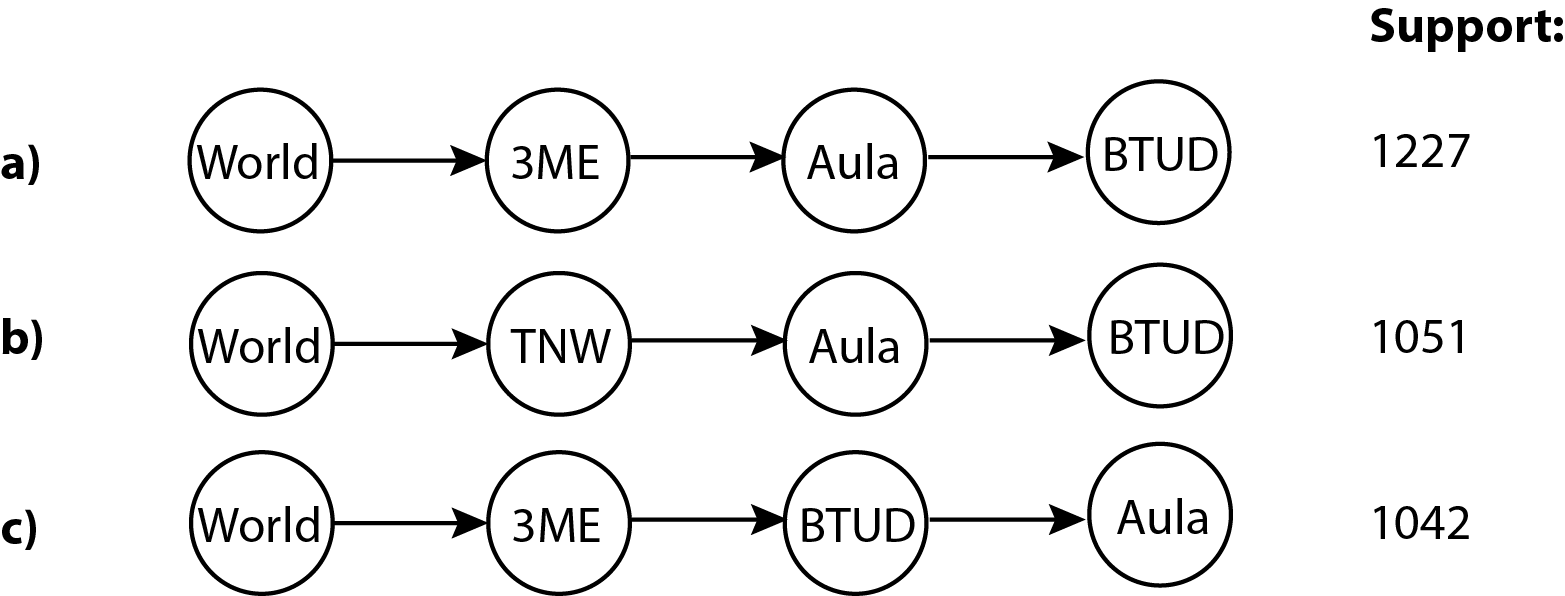
\includegraphics[scale=0.7]{length-4-pattern.png}
\captionsetup{justification=centering}
\caption{trajectory pattern with support > 1000 and four distinct locations}
\label{figure:len4pattern}
\end{figure}

These three movement patterns from users of the TU Delft Campus are visualized on the map in \autoref{figure:patternAmap}, \autoref{figure:patternBmap} and \autoref{figure:patternCmap}.

\begin{figure}[H]
\centering
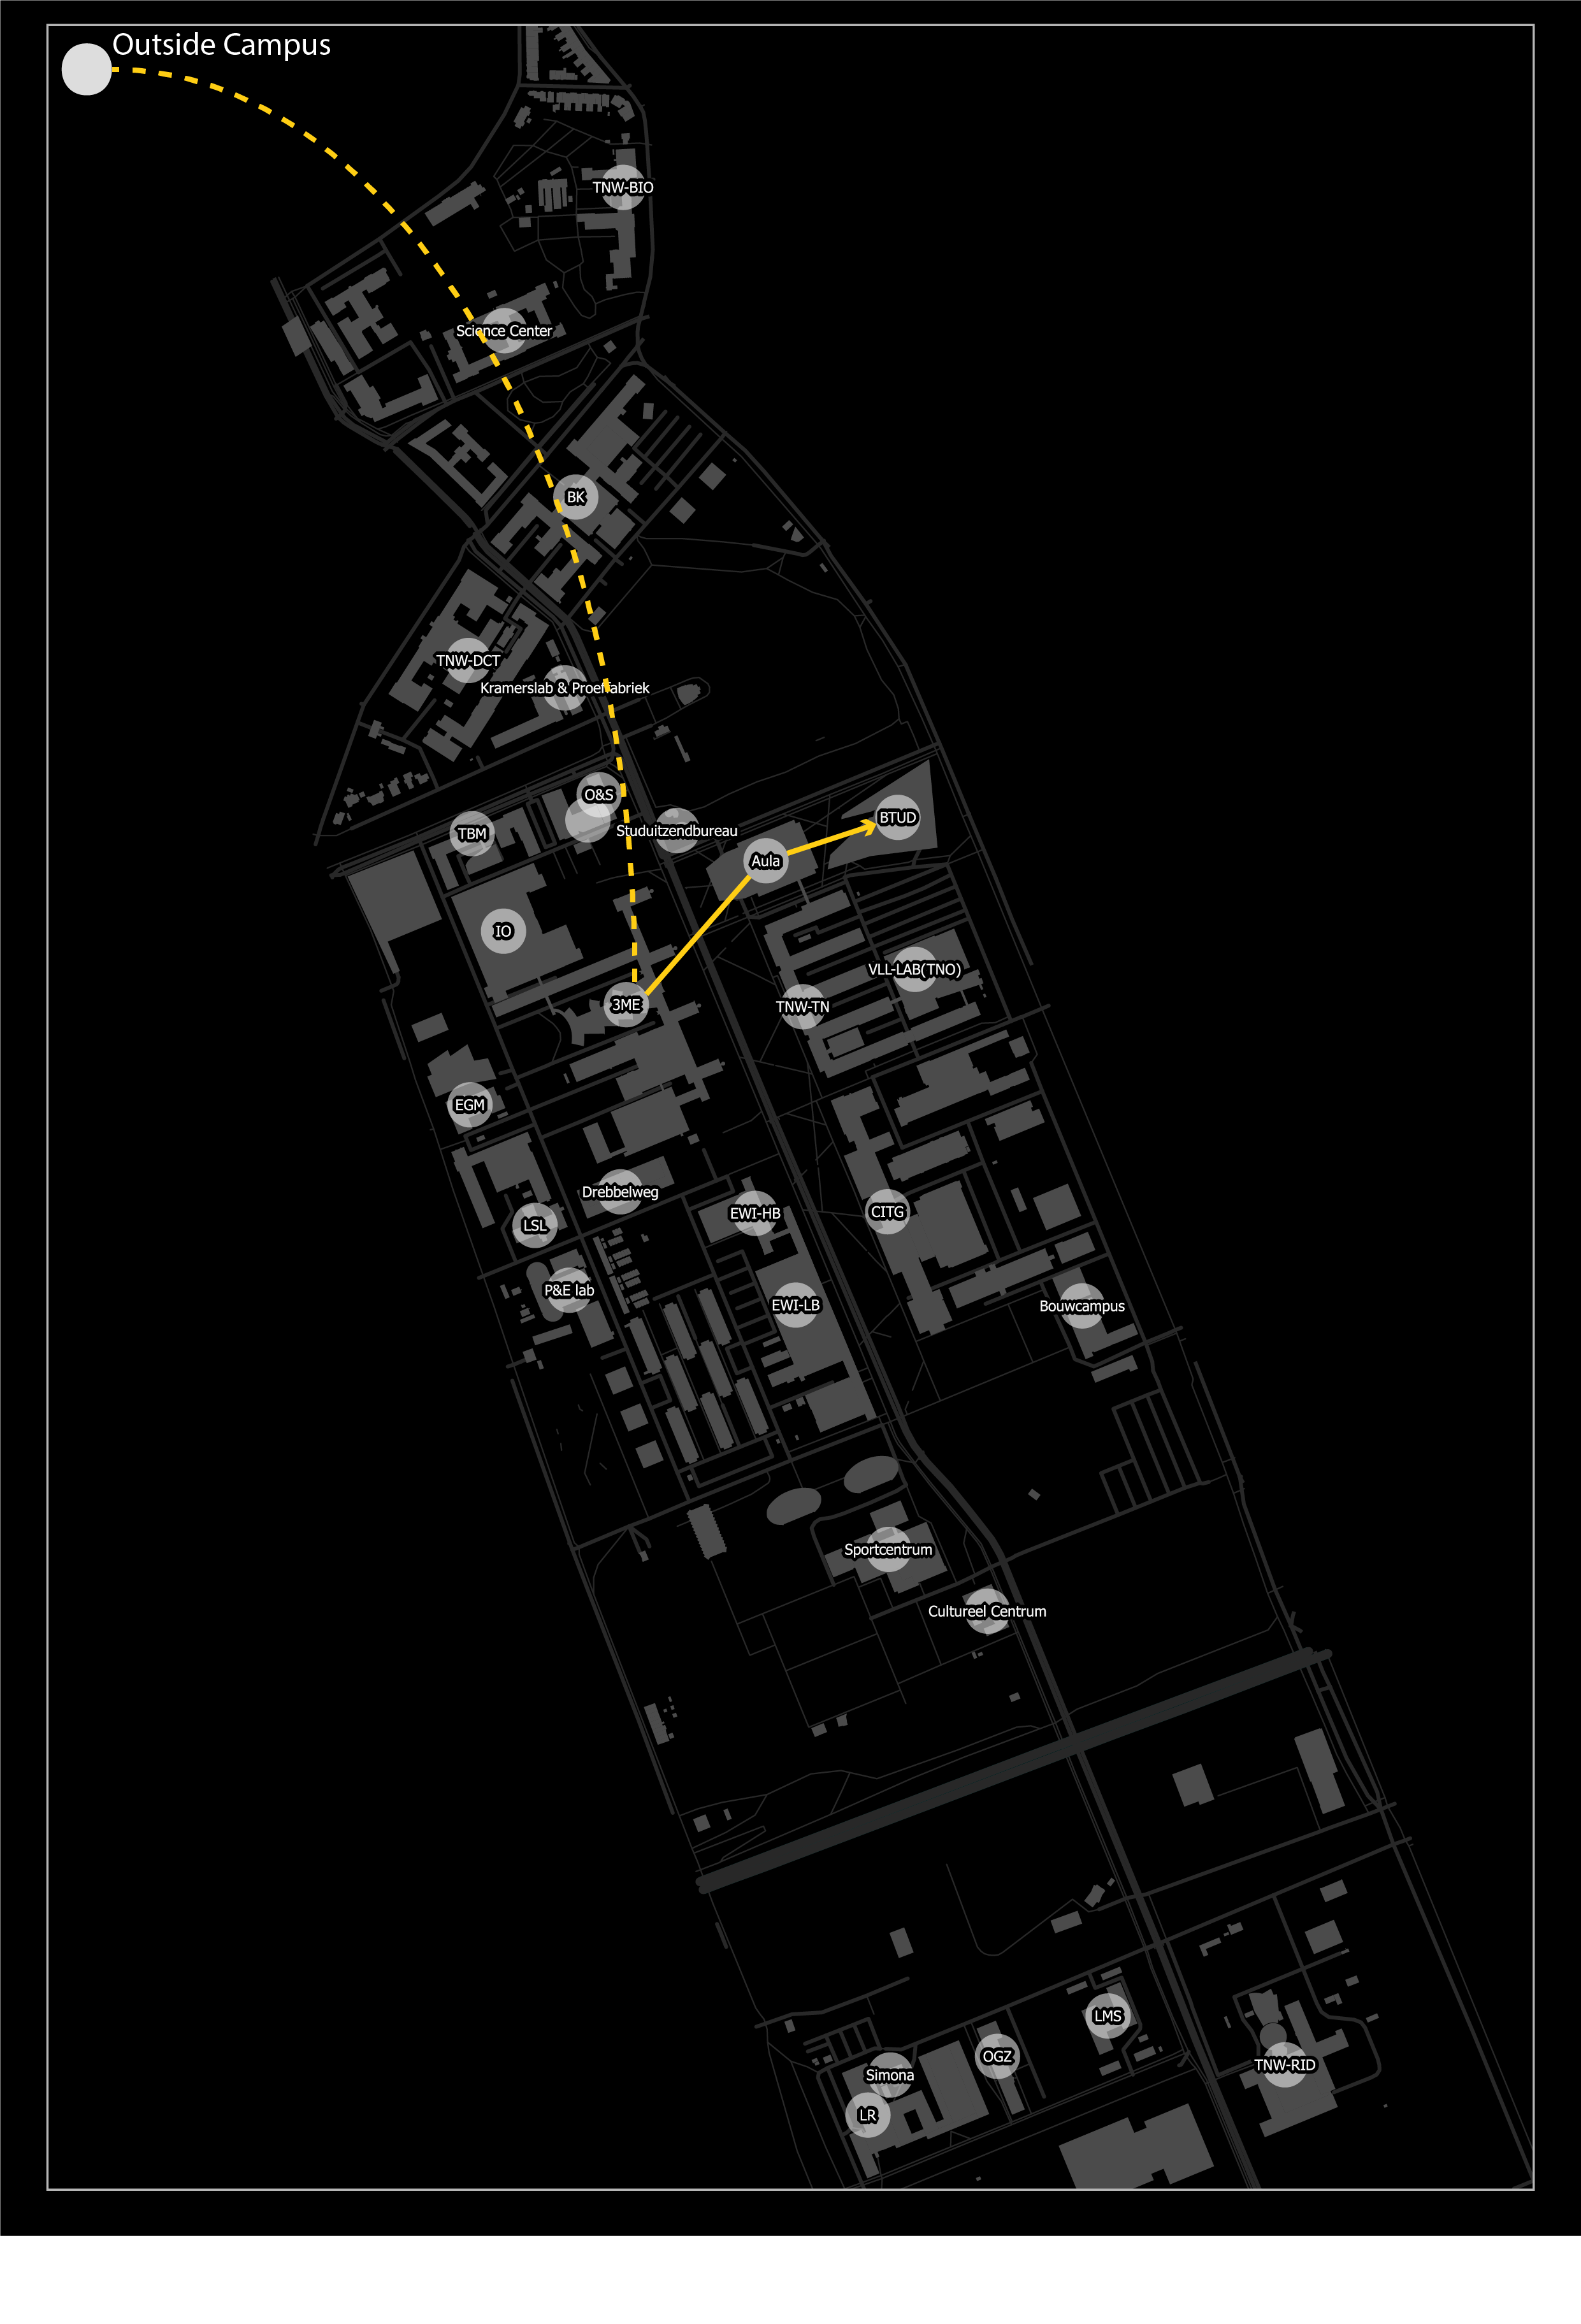
\includegraphics[scale=0.7]{patterna.png}
\captionsetup{justification=centering}
\caption{Trajectory pattern A, $$world\rightarrow 3me \rightarrow aula \rightarrow btud$$}
\label{figure:patternAmap}
\end{figure}

\begin{figure}[H]
\centering
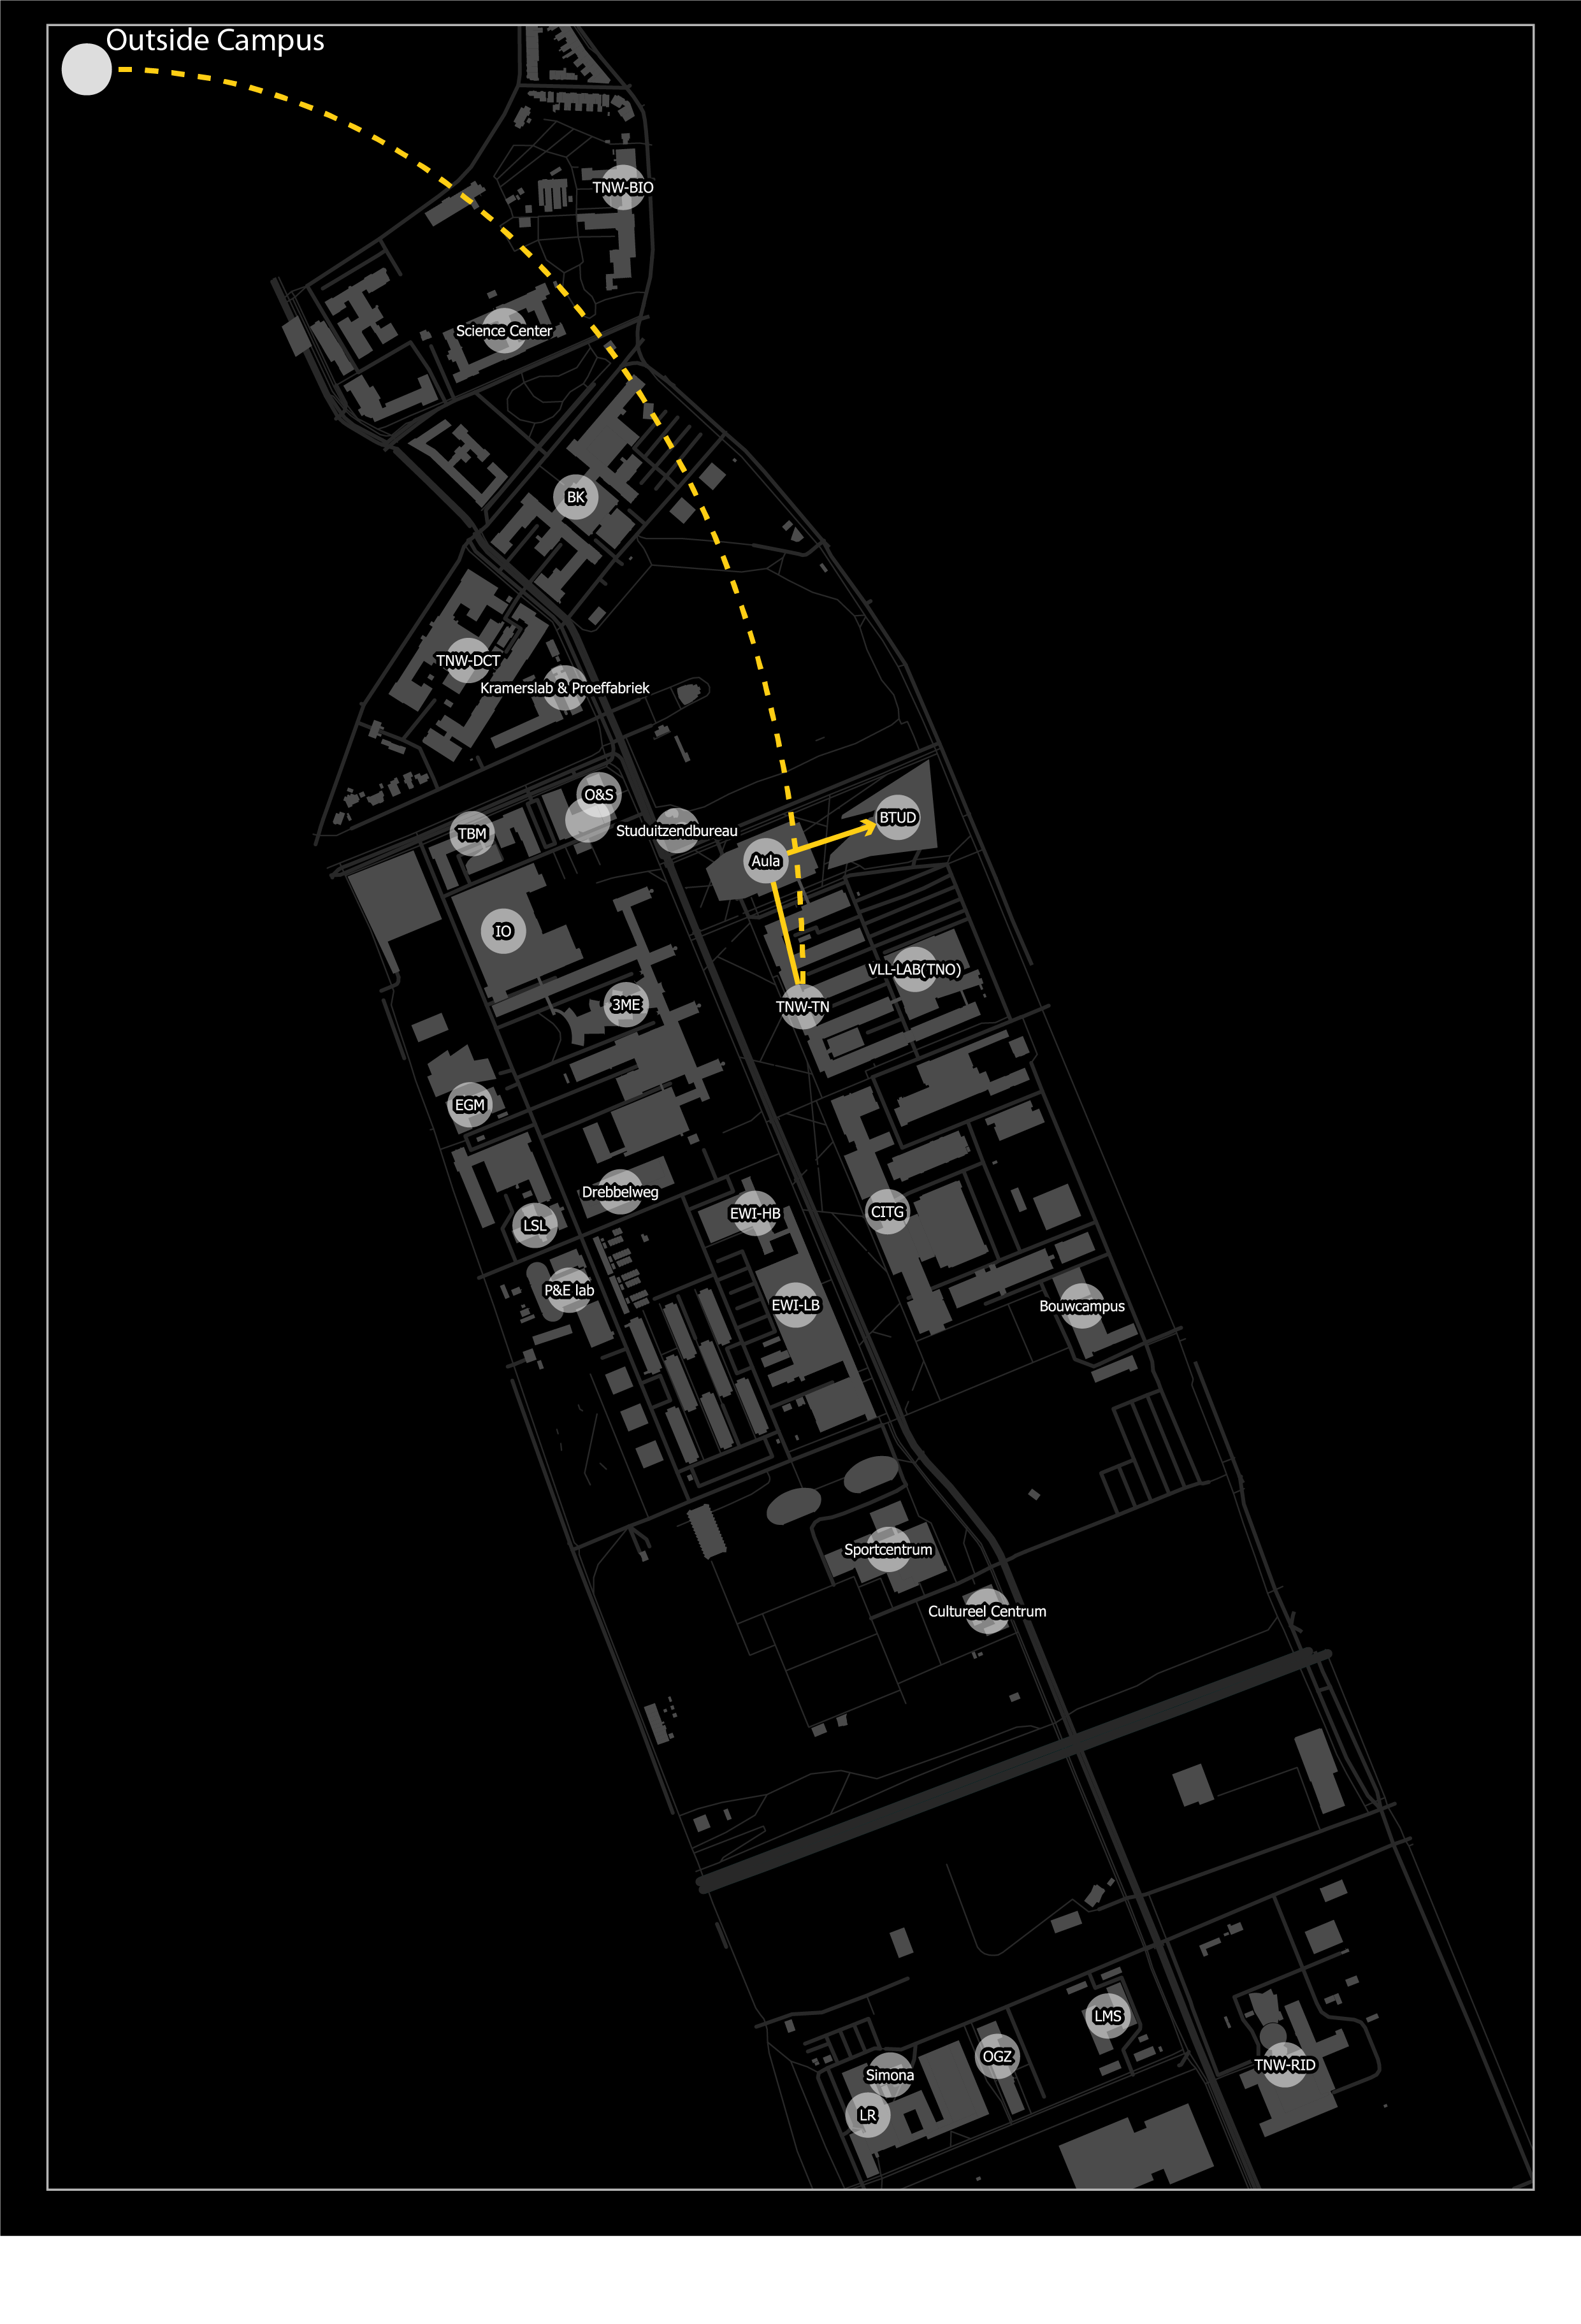
\includegraphics[scale=0.7]{patternb.png}
\captionsetup{justification=centering}
\caption{Trajectory pattern B, $$world\rightarrow tnw \rightarrow aula \rightarrow btud$$}
\label{figure:patternBmap}
\end{figure}

\begin{figure}[H]
\centering
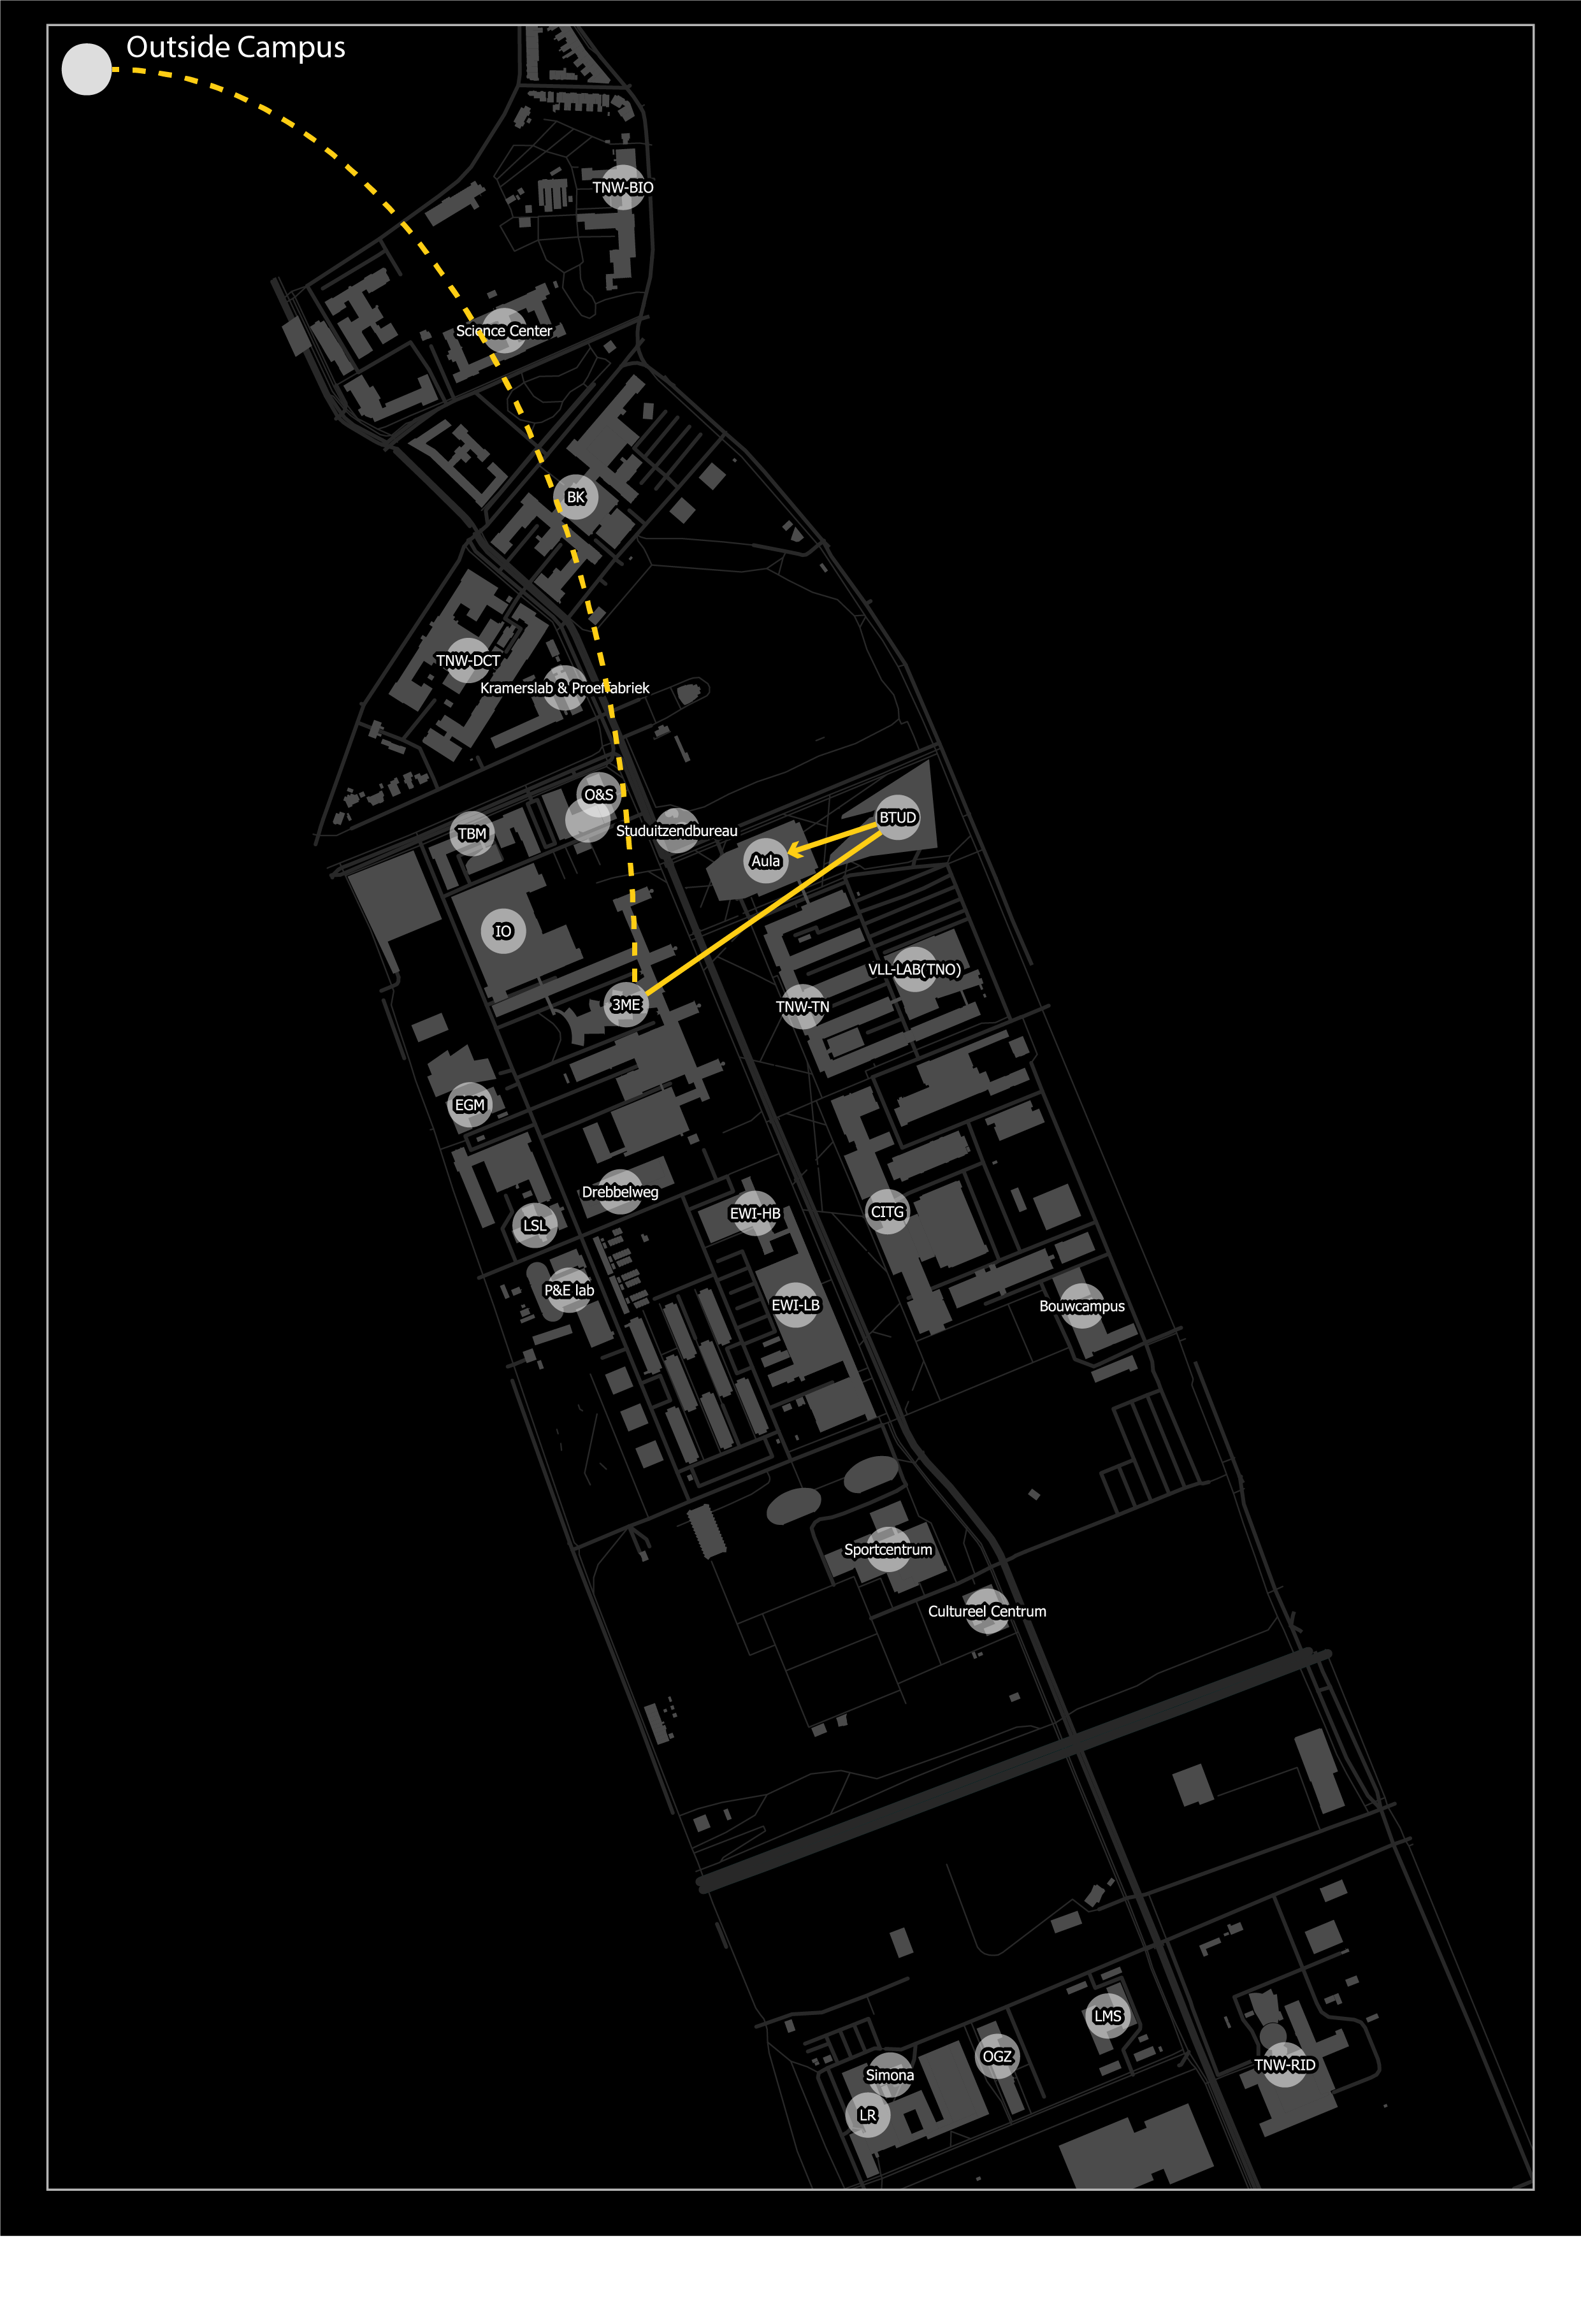
\includegraphics[scale=0.7]{patternc.png}
\captionsetup{justification=centering}
\caption{Trajectory pattern C, $$world\rightarrow 3me \rightarrow btud \rightarrow aula$$}
\label{figure:patternCmap}
\end{figure}

\subsection{Trajectory filtering}
Trajectories can serve another purpose. Although a splitting threshold of 5.5 hours was used, we noticed numerous trajectories with a temporal granularity of more than one day. Considering human life patterns, and mobile devices are for this research related to people, trajectories should present human behaviour. This means that people usually come to work in the morning, leave in the evening to go home and sleep during the night. Trajectories that are stretched over more than one day do not illustrate human behaviour, as the mobile devices do not leave the 'working environment' to go home and sleep. Besides a longer time interval of several trajectories, they also show a systematic pattern in there states. Only by creating trajectories and based on knowledge of human movement behaviour, can these trajectories be filtered out. 
